\chapter{Propagator and joint probability distribution in the position basis}

\section{General theory for the propagator of two particles}

\subsection{Non-interacting systems}

The propagator for a single particle system is used to find the probability distribution $\tilde{P}(x)$ of a state at anytime, i.e., for a state $\ket{\psi(t_0)}$ of a single particle,
\begin{equation}
    \tilde{P}(q_F, t_F) = \braket{q_F}{\psi(t_F)} = \int K(q_F, q_0; \Dd{t})\psi(q_0, t_0)\dd{q_0}.
\end{equation}
The probability of finding the particle at any point $(q_F, t_F)$ in spacetime is defined as
\begin{equation}
    P(q_F, t_F) \equiv |\tilde{P}(q_F, t_F)|^2
\end{equation}
This idea can be easily extended to describe any multiparticle system. But we shall only concern two particles systems in this study. Because the conventional notation is quite cumbersome, I shall introduce my own concise notation. From now on, every unprimed variable belong to particle one, and every unprimed variable, to particle one. E.g., the first particle Hilbert space shall be written with $\hilb$, and for the second particle, $\hilb_2$. This extends to all physical variables, e.g., position and momenta. The combined state shall be referred as $\eta$, and the separate states as $\xi$. Note that primed time do not exist; the interaction must happen simultaneously at a point in time; therefore, all the time variables $t$ will not be primed.

Let there be a combined state ket of two subsystems $\ket{\eta}$. If $\eta$ is separable at any point in time $t_0$, it follows that
\begin{equation}
    \ket{\eta} = \ket{\xi} \tensor \ket{\xi'}.
\end{equation}
If there are no interactions between the subsystems following $t_0$, the Hamiltonian operator must be separable which also implies that the time evolution operator $\hat{U}$ is also separable. From the property of tensor product, the quantity $\braket{q, q'}{\eta(t_0)}$ can be written as
\begin{equation}
    \braket{q, q'}{\eta(t_0)} = \left[\bra{q} \tensor \bra{q'}\right]\left[\ket{\xi} \tensor \ket{\xi'}\right] = \braket{q}{\xi(t_0)}\braket{q'}{\xi'(t_0)} = \xi(q, t_0)\xi'(q', t_0),
\end{equation}
which represents the product of the probability that $\xi$ is at $(q, t_0)$, and $\xi'$ is at $q', t_0$. We call $\braket{q, q'}{\eta(t_0)}$, the \textbf{joint probability distribution}. The modulus squared of the joint probability distribution gives the \textbf{joint probability amplitude}, $|\braket{q, q'}{\eta(t_0)}|^2$ which represents the probability to find $\xi$ at $(q, t_0)$ and $\xi'$ at $(q', t_0)$.

In the position basis, the joint probability amplitude is a function that takes in the position of both particles and outputs the probability that both $\xi$ and $\xi'$ will be there. Therefore, the joint probability amplitude encodes a surface, which can be plotted as shown in \cref{fig:jpddemonstration}. The probability amplitude of each particle can be found by projecting the surface onto the axis of each corresponding position basis.
\begin{figure}
    \centering
    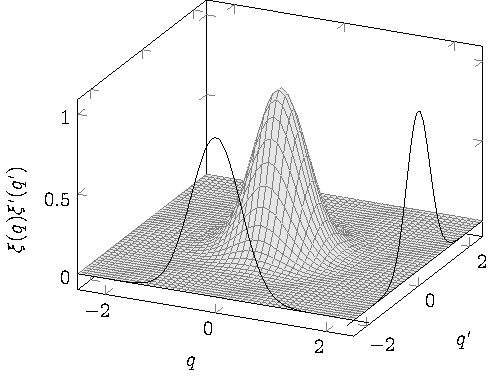
\includegraphics{diagrams/jpddemonstration}
    \caption{Example of the joint probability amplitude of a Gaussian wave packet.}
    \label{fig:jpddemonstration}
\end{figure}

\subsection{Interacting systems}

Let there be a state ket $\ket{\eta}$ which describes the quantum state of two particles. When the two particles are interacting, the time-evolution operator cannot be factored into tensor products of two operators. Therefore, there can only be one combined time-evolution operator for both of the systems:
\begin{equation}
    \hat{U}(t_F, t_0) = \exp[-\im\Dd{t}\left(\frac{\hat{p}^2}{2m} + \frac{\hat{p}'^2}{2m'} + V(\hat{q}, \hat{q}', t)\right)]
\end{equation}
The consequence of the combined time-evolution operator is that, we cannot calculate the joint probability distribution between different time of the subsystem. For simplicity’ sake, let the index $j = i + 1$, where $t_j = t_i + \Dd{t}$ in which $\Dd{t} \appr 0$.
\begin{align}
    &\braket{q_j, q_j'}{\eta(t_j)} \\
    &= \mel{q_j, q_j'}{\hat{U}(t_j, t_i)}{\eta(t_i)}. \\
    &= \iint \dd{q_i}\dd{q_i'} \mel{q_j, q_j'}{\hat{U}(t_j, t_i)}{q_i, q_i'}\braket{q_i, q_i'}{\eta(t_i)}.
\end{align}

As seen, the form of transition element is
\begin{equation}
    \mel{q_j, q_j'}{\exp[-\im\Dd{t}\left(\frac{\hat{p}^2}{2m} + \frac{\hat{p}'^2}{2m'} + V(\hat{q}, \hat{q}', t)\right)]}{q_i, q_i'}.
\end{equation}
The terms in the exponents can be separated due to the vanishing commutator when $\Dd{t} \appr 0$. By separating the terms in the exponents and inserting two complete sets of momentum basis, the equation above turns into
\begin{align}
    & \frac{1}{(2\cpi)^2} \iint\dd{p}\dd{p'} \mel*{q_j, q_j'}{\exp[-\im\Dd{t}\frac{\hat{p}^2}{2m}]}{p, p'}\mel{p, p'}{\exp[-\im\Dd{t}\frac{\hat{p}'^2}{2m'}]\exp[-\im\Dd{t}V(\hat{q}, \hat{q}', t)]}{q_i, q_i'} \nonumber\\
    &= \frac{1}{(2\cpi)^2} \iint\dd{p}\dd{p'} \exp[-iu\Dd{t}\left(\frac{p^2}{2m} + \frac{p'^2}{2m'} + V(q_i, q_i, \Dd{t})\right)]\braket{q_j}{p}\braket{q_j'}{p'}\braket{q_i}{p}\conj\braket{q_j'}{p'}\conj \nonumber\\
    &= \frac{1}{(2\cpi)^4} \e^{-\im\Dd{t}V(q_i, q_i', t)} \int\dd{p}\exp[-\im\Dd{t}\frac{p^2}{2m} + \im p(q_j - q_i)]\int\dd{p'}\exp[-\im\Dd{t}\frac{p'^2}{2m'} + \im p'(q_j' - q_i')^2] \nonumber\\
    &= \frac{(mm')^{\frac{1}{2}}}{8\cpi^3\im\Dd{t}}\exp[-\im\Dd{t}V(q_i, q_i', t) + \frac{\im m'}{2\Dd{t}}(q_j' - q_i')^2 + \frac{\im m}{2\Dd{t}}(q_j - q_i)^2].
\end{align}
To find the propagator for an interacting system, we need to perform successive integrals on $q$ and $q'$, i.e.,
\begin{equation}
    K_{\eta} = \idotsint \dd{q_N}\dd{q_N'}\dots\dd{q_1}\dd{q_1'}\mel{q_F, q_F'}{\hat{U}(t_F, t_N)}{q_N, q_N'}\dots\mel{q_1, q_1'}{\hat{U}(t_1, t_0)}{q_0, q_0'}
\end{equation}

Notice that when there is no interaction between the two systems ($V = 0$), the integrals become separable and reduces down to the form of the non-interacting system's propagator but off by a normalization factor.

There are two common forms of interaction, which is the spring interaction and the coulomb interaction. Both of which includes the term $(q_i - q_i')^2$ in $V(q, q')$, which causes major problems in integration. When expanded, there is a $q_iq_i'$ term that makes the integral inseparable which causes the integral pattern to not repeat; therefore, we resort to perturbation.

\subsection{Form of the two particle perturbation series}

The perturbation series for one particle are already given by Feynman in his path integrals textbook:
\begin{equation}
    K_n(F, 0) = \left(-\im\right)^n\idotsint K_0(F, n)\prod_{i = 1}^n V(i)K_0(i, i - 1)\dd{\tau_i}
\end{equation}
where $K_n$ is the $n$'th order perturbation, $K(j, k) = K(q_j, t_j; q_k, t_k)$, $K = \ssum_nK_n$ and $\dd{\tau_i} = \dd{q_i}\dd{q_i}\dd{t_i}$. To apply it with two particles, we extend it:
\begin{equation}
    K_n(F, 0; F', 0') = \left(-\im\right)^n\idotsint K_0(F, n)K_0(F', n')\left[\prod_{i = 1}^nV(i)K_0(i, i - 1)K_0(i', i' - 1)\dd{q_i}\dd{q_i'}\dd{t_i}\right]. \label{eq:generaltwoparticleperturbation}
\end{equation}
We can also expand the joint probability distribution in the form of the perturbation series.
\begin{align}
    \eta(q_F, q_F'; t_F) &= \int K(q_F, q_F'; q_0, q_0'; t_F - t_0)\eta(q_0, q_0'; t_0)\dd{q_0}\dd{q_0'} \\
    &= \int \sum_n K_n(q_F, q_F'; q_0, q_0'; t_F - t_0)\eta(q_0, q_0'; t_0) \dd{q_0}\dd{q_0'} \\
    &= \sum_n \int K_n(q_F, q_F'; q_0, q_0'; t_F - t_0)\eta(q_0, q_0'; t_0) \dd{q_0}\dd{q_0'}
\end{align}

\section{Initial states of choice}
\label{sec:initial_states_of_choice}

From now on, I shall use the letter $\xi$ to refer to a state of a single particle, and the letter $\eta$ to refer to the combined state of two particles.

We are interested in the time evolution of a Gaussian wave packet due to its mathematical simplicity. The normalized state of a Gaussian wave packet is given by
\begin{equation}
    \sqrt[4]{\frac{1}{2\cpi\sigma}}\exp[\im p q - \frac{(q - s)^2}{4\sigma^2}]. \label{eq:unentangled_state}
\end{equation}
For two separable particles, its joint probability is
\begin{align}
    \braket{q, q'}{\eta(t_0)} &= \sqrt[4]{\frac{1}{2\cpi\sigma^2}}\sqrt[4]{\frac{1}{2\cpi\sigma'^2}}\exp[\im pq - \frac{(q - s)^2}{4\sigma^2}]\exp[\im p'q' - \frac{(q' - s')^2}{4\sigma'^2}] \\
    &= \sqrt{\frac{1}{2\cpi\sigma\sigma'}}\exp[\im pq - \frac{(q - s)^2}{4\sigma^2}]\exp[\im p'q' - \frac{(q' - s')^2}{4\sigma'^2}]
\end{align}

As we'll see, the higher order perturbation terms (at least of the spring system) are expressed as the integral of the product between the wave function and some polynomials, which we'll find later.
\begin{align}
    &\braket{q}{\xi(t)} \\ &= \int K_0(q_F, q_0;t_F)\braket{q_0}{\xi(t)}\dd{q_0} \\
    &= \sqrt{\frac{m}{2\cpi\im t_F}}\int\exp[\frac{\im m}{2t_F}(q_F - q_0)^2] \left(\sqrt[4]{\frac{1}{2\cpi\sigma}}\exp[\im p q_0 - \frac{(q_0 - s)^2}{4\sigma^2}]\right)\dd{q_0} \\
    &= \sqrt[4]{-\frac{m^2}{8\cpi^3t_F^2\sigma^2}}\int\exp[\frac{\im m}{2t_F}(q_F - q_0)^2 + \im p q_0 - \frac{(q_0 - s)^2}{4\sigma^2}]\dd{q_0} \\
    &= \sqrt[4]{-\frac{m^2}{8\cpi^3t_F^2\sigma^2}}\int\exp[\left(\frac{\im m q_F^2}{2t_F} - \frac{s^2}{4\sigma^2}\right) + q\left(-\frac{\im m q_F}{t_F} + \im p + \frac{s}{2\sigma^2}\right) + q^2\left(\frac{\im m}{2t_F} - \frac{1}{4\sigma^2}\right)]\dd{q_0} \\
    &= \sqrt[4]{-\frac{m^2}{8\cpi^3t_F^2\sigma^2}} \cdot 2\sigma\sqrt{\frac{\cpi t_F}{-2\im m\sigma^2 + t_F}}\exp[\frac{4 \im m p q_{F} σ^{2} - m q_{F}^{2} + 2 m q_{F} s - m s^{2} - 2 \im p^{2} t_{F} σ^{2} - 2 p s t_{F}}{4 m σ^{2} + 2 \im t_{F}}]  \nonumber\\
    &= \sqrt[4]{\frac{2m^2\sigma^2}{\cpi(2m\sigma^2 + \im t_F)^2}}\exp[\frac{4 \im m p q_{F} σ^{2} - m q_{F}^{2} + 2 m q_{F} s - m s^{2} - 2 \im p^{2} t_{F} σ^{2} - 2 p s t_{F}}{4 m σ^{2} + 2 \im t_{F}}].
\end{align}
To plot its probability amplitude, we have to take its modulus squared, which equals to
\begin{equation}
    \frac{m σ}{\sqrt{4 m^{2} σ^{4} + t_{F}^{2}}}\exp[\frac{- 2 m^{2} q_{F}^{2} σ^{2} + 4 m^{2} q_{F} s σ^{2} - 2 m^{2} s^{2} σ^{2} + 4 m p q_{F} t_{F} σ^{2} - 4 m p s t_{F} σ^{2} - 2 p^{2} t_{F}^{2} σ^{2}}{4 m^{2} σ^{4} + t_{F}^{2}}]
\end{equation}

\section{The spring system}

The spring potential is given by $V(q, q') = \frac{k}{2}(q - q')^2$. I shall let $\alpha = \frac{k}{2}$ to simplify the notation a bit.

\subsection{First order perturbation term}
\label{sec:spring_1storder}

From \cref{eq:generaltwoparticleperturbation}, set $t_1 = t, t_0 = 0$
\begin{align}
    &K_1(F, 0; F', 0) \nonumber \\
    &= \left(-\im\right)^1\iiint K_0(F, 1)K_0(F', 1')K_0(1, 0)K_0(1, 0')\alpha(q_1 - q_1')^2\dd{q_1}\dd{q_1'}\dd{t}. \\
    &= -\im\alpha\int_0^{t_F}\left[\iint K_0(q_F, q_1; t_F - t)K_0(q_F', q_1'; t_F - t)K_0(q_1, q_0; t)K_0(q_1', q_0'; t)(q_1 - q_1')^2\dd{q_1}\dd{q_1'}\right]\dd{t}. \nonumber
\end{align}
We then let the terms in the square bracket,
\begin{equation}
    \iint K_0(q_F, q_1; t_F - t)K_0(q_F', q_1'; t_F - t)K_0(q_1, q_0; t)K_0(q_1', q_0'; t)(q_1 - q_1')^2\dd{q_1}\dd{q_1'}
\end{equation}
equals $I$; therefore, $K_1 = -\im\alpha\int_0^{t_F} I\dd{t}$.

We then separate $I$ into three integrals:
\begin{gather}
    I_{P1} = \int q_1^2K_0(q_F, q_1; t_F - t)K_0(q_1, q_0; t)\dd{q_1} \int K_0(q_F', q_1'; t_F - t)K_0(q_1', q_0'; t)\dd{q_1'}, \label{eq:spring_IP1}\\
    I_{P2} = \int K_0(q_F, q_1; t_F - t)K_0(q_1, q_0; t)\dd{q_1} \int q_1'^2K_0(q_F', q_1'; t_F - t)K_0(q_1', q_0'; t)\dd{q_1'}, \label{eq:spring_IP2}\\
    I_{P3} = \int q_1K_0(q_F, q_1; t_F - t)K_0(q_1, q_0; t)\dd{q_1} \int q_1'K_0(q_F', q_1'; t_F - t)K_0(q_1', q_0'; t) \dd{q_1'} \label{eq:spring_IP3},
\end{gather}
where $I = I_{P1} + I_{P2} + 2I_{P3}$. The integrals without the factor $q_1$ and $q_1^2$ can be reduced into the kernel for the free particle:
\begin{gather}
    I_{P1} = K_0(q_F', q_0'; t_F)\int q_1^2K_0(q_F, q_1; t_F - t)K_0(q_1, q_0; t)\dd{q_1} \\
    I_{P2} = K_0(q_F, q_0; t_F)\int q_1'^2 K_0(q_F', q_1'; t_F - t)K_0(q_1', q_0'; t)\dd{q_1'}
\end{gather}
Since $I_{P2}$ can be obtained by switching all the primed variables with the corresponding unprimed in $I_{P1}$, we're left with two family of integrals:
\begin{equation}
    \int q_1K_0(q_F, q_1; t_F - t)K_0(q_1, q_0; t)\dd{q_1} \mathand \int q_1^2K_0(q_F, q_1; t_F - t)K_0(q_1, q_0; t)\dd{q_1}. \label{eq:spring_family_of_integrals}
\end{equation}
To evaluate these, we first simplify the product of kernel under the assumption that $t_F > t$.
\begin{align}
    &K_0(q_F, q_1; t_F - t)K_0(q_1, q_0; t) \nonumber\\
    &= \sqrt{\frac{m}{2\cpi\im(t_F - t)}}\sqrt{\frac{m}{2\cpi\im t}}\exp[\frac{\im m}{2(t_F - t)}(q_F - q_1)^2 + \frac{\im m}{2t}(q_1 - q_0)^2] \\
    &= \frac{m}{2\cpi}\sqrt{-\frac{1}{t(t_F - t)}} \exp[q_1^2\left(\frac{\im m}{2t} + \frac{\im m}{2(t_F - t)}\right) - q_1\left(\frac{\im m q_0}{t} + \frac{\im m q_F}{t_F - t}\right) + \left(\frac{\im m q_0^2}{2t} + \frac{\im m q_F^2}{2(t_F - t)}\right)] \nonumber \\
    &= \frac{m}{2\cpi}\sqrt{-\frac{1}{t(t_F - t)}} \exp[-q_1^2\left(\frac{m t_F}{2\im t(t_F - t)}\right) - q_1(\im m)\left(\frac{q_0}{t} + \frac{q_F}{t_F - t}\right) - \left(\frac{m}{2\im}\right)\left(\frac{q_0^2}{t} + \frac{q_F^2}{t_F - t}\right)] \nonumber
\end{align}
The normalization factor are pulled out. Both integrals in \cref{eq:spring_family_of_integrals} can be evaluated with
\begin{equation}
    a = \frac{m t_F}{2\im t(t_F - t)}, \quad b = \im m\left(\frac{q_0}{t} + \frac{q_F}{t_F - t}\right) \mathand c = \left(\frac{m}{2\im}\right)\left(\frac{q_0^2}{t} + \frac{q_F^2}{t_F - t}\right)
\end{equation}
in which,
\begin{equation}
    \exp[\frac{b^2}{4a} - c] = \exp[\frac{\im m}{2t_F}(q_F - q_0)^2] = \sqrt{\frac{2\cpi\im t_F}{m}}K_0(q_F, q_0; t_F).
\end{equation}
To summarize,
\begin{align}
    \int q_1K_0(q_F, q_1; t_F - t)K_0(q_1, q_0; t)\dd{q_1} &= -\frac{b}{2}\sqrt{\frac{\cpi}{a^3}}\times\frac{m}{2\cpi}\sqrt{-\frac{1}{t(t_F - t)}}\times\sqrt{\frac{2\cpi\im t_F}{m}}K_0(q_F, q_0; t_F) \nonumber\\
    &= -\frac{b}{2}\sqrt{\frac{\cpi}{a^3}} \times \sqrt{\frac{mt_F}{2\cpi\im t(t_F - t)}}K_0(q_F, q_0; t_F), \label{eq:spring_deg1gaussian_form}
\end{align}
and
\begin{equation}
    \int q_1^2K_0(q_F, q_1; t_F - t)K_0(q_1, q_0; t)\dd{q_1} = \frac{1}{4}\sqrt{\frac{\cpi}{a^5}}(2a + b^2) \times \sqrt{\frac{mt_F}{2\cpi\im t(t_F - t)}}K_0(q_F, q_0; t_F). \label{eq:spring_deg2gaussian_form}
\end{equation}

On the Gaussian integral with degree one,
\begin{equation}
    -\frac{b}{2}\sqrt{\frac{\cpi}{a^3}} = \sqrt{\frac{2\cpi t}{mt_F^3}}\frac{\sqrt{-\im(t_F - t)^3}}{\im(t_F - t)} \times \left[q_0(t_F - t) + q_Ft\right];
\end{equation}
thus from \cref{eq:spring_deg1gaussian_form},
\begin{align}
    \int q_1K_0(q_F, q_1; t_F - t)K_0(q_1, q_0; t) &= \begin{multlined}[t]
        \sqrt{\frac{2\cpi t}{mt_F^3}}\frac{\sqrt{-\im(t_F - t)^3}}{\im(t_F - t)} \times \left[q_0(t_F - t) + q_Ft\right] \\
        \times \sqrt{\frac{mt_F}{2\cpi\im t(t_F - t)}}K_0(q_F, q_0; t_F)
    \end{multlined} \\
    &= -\frac{1}{t_F}\left[q_0(t_F - t) + q_Ft\right]K_0(q_F, q_0; t_F).
\end{align}
On the Gaussian integral with degree two,
\begin{equation}
    \frac{1}{4}\sqrt{\frac{\cpi}{a^5}}(2a + b^2) = -\sqrt{\frac{2\cpi t}{m^3t_F^5}}\frac{\sqrt{\im(t_F - t)^5}}{(t_F - t)^2}\left[m\left(q_0(t_F - t) + q_Ft\right)^2 + \im tt_F(t_F - t)\right];
\end{equation}
and thus,
\begin{align}
    &\int q_1^2K_0(q_F, q_1; t_F - t)K_0(q_1, q_0; t)\dd{q_1} \\
    &= \sqrt{\frac{mt_F}{2\cpi\im t(t_F - t)}}K_0(q_F, q_0; t_F)  \times -\sqrt{\frac{2\cpi t}{m^3t_F^5}}\frac{\sqrt{\im(t_F - t)^5}}{(t_F - t)^2}\left[m\left(q_0(t_F - t) + q_Ft\right)^2 + \im tt_F(t_F - t)\right] \nonumber\\
    &= -\frac{1}{mt_F^2}\left[m\left(q_0(t_F - t) + q_Ft\right)^2 + \im tt_F(t_F - t)\right]K_0(q_F, q_0; t_F).
\end{align}

We're now in the place to finally construct the first order propagator term for the spring system. Recall that
\begin{equation}
    K_1 = -\im\alpha\int_0^{t_F} I\dd{t} = -\im\alpha\left[\int_0^{t_F}I_{P1}\dd{t} + \int_0^{t_F}I_{P2}\dd{t} + 2\int_0^{t_F}I_{P3}\dd{t}\right]
\end{equation}
From earlier,
\begin{gather}
    \begin{aligned}
        I_{P1} &= K_0(q_F', q_0'; t_F)\int q_1^2K_0(q_F, q_1; t_F - t)K_0(q_1, q_0; t)\dd{q_1} \\
        &= -\frac{1}{mt_F^2}\left[m\left(q_0(t_F - t) + q_Ft\right)^2 + \im tt_F(t_F - t)\right]K_0(q_F, q_0; t_F)K_0(q_F', q_0'; t_F),
    \end{aligned}
    \\
    \begin{aligned}
        I_{P2} &= K_0(q_F, q_0; t_F)\int q_1'^2 K_0(q_F', q_1'; t_F - t)K_0(q_1', q_0'; t)\dd{q_1'} \\
        &= -\frac{1}{mt_F^2}\left[m\left(q_0'(t_F - t) + q_F't\right)^2 + \im tt_F(t_F - t)\right]K_0(q_F, q_0; t_F)K_0(q_F', q_0'; t_F),
    \end{aligned}
    \\
    \begin{aligned}
        I_{P3} &= -\frac{1}{t_F}\left[q_0(t_F - t) + q_Ft\right]K_0(q_F, q_0; t_F) \times -\frac{1}{t_F}\left[q_0'(t_F - t) + q_F't\right]K_0(q_F', q_0'; t_F) \\
        &= \frac{1}{t_F^2}\left[q_0(t_F - t) + q_Ft\right]\left[q_0'(t_F - t) + q_F't\right]K_0(q_F, q_0; t_F)K_0(q_F', q_0'; t_F).
    \end{aligned}
\end{gather}
Thus,
\begin{multline}
    K_1 = -\im\alpha K_0(q_F, q_0; t_F)K_0(q_F', q_0'; t_F) \frac{1}{t_F^2} \left[-\frac{1}{m}\int_0^{t_F}m\left(q_0(t_F - t) + q_Ft\right)^2 + \im tt_F(t_F - t)\dd{t} \right. \\
    -\frac{1}{m}\int_0^{t_F}m\left(q_0'(t_F - t) + q_F't\right)^2 + \im tt_F(t_F - t)\dd{t} \\
    \left. + \int_0^{t_F}\left[q_0(t_F - t) + q_Ft\right]\left[q_0'(t_F - t) + q_F't\right]\dd{t}\right]
\end{multline}
The integrals are then taken out to be evaluated term by term. Since the integrand of these integrals are all polynomials, we can just plug it into \texttt{SymPy.jl}:
\begin{gather}
    \int_0^{t_F}m\left(q_0(t_F - t) + q_Ft\right)^2 = \frac{t_F^3}{6}\left(2m(q_0 + q_F)^2 + \im t_F\right) \\
    \int_0^{t_F}m\left(q_0'(t_F - t) + q_F't\right)^2 = \frac{t_F^3}{6}\left(2m(q_0' + q_F')^2 + \im t_F\right) \\
    \int_0^{t_F}\left[q_0(t_F - t) + q_Ft\right]\left[q_0'(t_F - t) + q_F't\right]\dd{t} = \frac{t_F^3}{6}\left(2q_0q_0' + q_0q_F' + q_0'q_F + 2q_Fq_F'\right)
\end{gather}
Therefore, the first order perturbation term of the spring system takes the form
\begin{multline}
    K_1(q_F, q_0; q_F', q_0'; t_F) = -\im\frac{\alpha t_F}{6}K_0(q_F, q_0; t_F)K_0(q_F', q_0'; t_F) \\
    \times\left[-2\left(m(q_0 + q_F)^2 + m(q_0' + q_F')^2 + \im t_F\right) + 2q_0q_0' + q_0q_F' + q_0'q_F + 2q_Fq_F'\right]. \label{eq:spring_first_order_perturbation}
\end{multline}

\paragraph{Interpretation of the propagator} As of now, my knowledge of the propagator is pretty limited.

\subsection{Joint probability contribution from the first order perturbation term}

Let us first analyze the time evolution of a separable wave packet with the initial state
\begin{equation}
    \eta(q_0, q_0; t_0) \equiv \frac{1}{2\cpi\sqrt{\sigma\sigma'}}\exp[\im pq_0 + \im p'q_0' - \frac{(q_0 - s)^2}{4\sigma^2} - \frac{(q_0' - s')^2}{4\sigma'^2}].
\end{equation}
For simplicity's sake, let
\begin{gather*}
    \xi \equiv \exp[\im pq_0 - \frac{(q_0 - s)^2}{4\sigma^2}], \quad \xi' \equiv \exp[\im p'q_0' - \frac{(q_0' - s')^2}{4\sigma'^2}], \\
    K \equiv \sqrt{\frac{m}{2\cpi\im t_F}}\exp[\frac{\im}{2t_F}(q_F - q_0)^2], \quad K' \equiv \sqrt{\frac{m}{2\cpi\im t_F}}\exp[\frac{\im}{2t_F}(q_F' - q_0')^2].
\end{gather*}
Let us also set $t_0$ to be $0$. Using the first order perturbation term from \cref{eq:spring_first_order_perturbation}, the state at any following time $t_F$ is then
\begin{align}
    \eta(q_F, q_F'; t_F) &= \iint\left(K_0(q_F, q_0; q_F', q_0'; t_F - t_0) + K_1(q_F, q_0; q_F', q_0'; t_F - t_0)\right)\eta(q_0, q_0'; t_0)\dd{q}\dd{q_0'} \\
    &= \begin{multlined}[t]
        \frac{1}{2\cpi\sqrt{\sigma\sigma'}}\iint K_0(q_F, q_0; q_F', q_0'; t_F - t_0)\left\{1 - \im\frac{\alpha t_F}{6}\left[-2\left(m(q_0 + q_F)^2 \right.\right.\right.\\
        \left.\left.\left. + m(q_0' + q_F')^2 + \im t_F\right) + 2q_0q_0' + q_0q_F' + q_0'q_F + 2q_Fq_F'\right]\vphantom{\frac{\alpha t_F}{6}}\right\}
        \\ \exp[\im pq_0 + \im p'q_0' - \frac{(q_0 - s)^2}{4\sigma^2} - \frac{(q_0' - s')^2}{4\sigma'^2}]\dd{q_0}\dd{q_0'}
    \end{multlined} \\
    &= \begin{multlined}[t]
        \frac{1}{2\cpi\sqrt{\sigma\sigma'}}\iint KK'\xi\xi'\left\{1 - \im\frac{\alpha t_F}{6}\left[-2\left(m(q_0 + q_F)^2 \right.\right.\right.\\
        \left.\left.\left. + m(q_0' + q_F')^2 + \im t_F\right) + 2q_0q_0' + q_0q_F' + q_0'q_F + 2q_Fq_F'\right]\vphantom{\frac{\alpha t_F}{6}}\right\} \dd{q_0}\dd{q_0'}
    \end{multlined}
\end{align}
Note that this method of separation will work for all separable $\eta(t_0)$. Therefore, $\eta(t_0)$ doesn't have to be Gaussian: we just select it to be. The integral above can then be further expanded and broken down into smaller integrals:
\begin{align}
    \eta(q_F, q_F'; t_F) &= \begin{multlined}[t]
        \frac{1}{2\cpi\sqrt{\sigma\sigma'}}\left[\iint KK'\xi\xi'\dd{q_0}\dd{q_0'} \right.\\ \left.
        - \im\frac{\alpha t_F}{6}\iint KK'\xi\xi'\Big\{-2m(q_0^2 + 2q_0q_F + q_F^2 + q_0'^2 + 2q_0'q_F' + q_F'^2) \right.\\ \left.
        + 2q_0q_0' + 2q_Fq_F' + q_0q_F' + q_0'q_F + \im t_F\Big\}\dd{q_0}\dd{q_0'}  \vphantom{\iint}\right]
    \end{multlined} \\
\end{align}
I shall let $I$ equals the term in the big square bracket:
\begin{equation}
    I \equiv \begin{multlined}[t]
        \iint KK'\xi\xi'\dd{q_0}\dd{q_0'}
        - \im\frac{\alpha t_F}{6}\iint KK'\xi\xi'\Big\{-2m(q_0^2 + 2q_0q_F + q_F^2 + q_0'^2 + 2q_0'q_F' + q_F'^2) \\
        + 2q_0q_0' + 2q_Fq_F' + q_0q_F' + q_0'q_F + \im t_F\Big\}\dd{q_0}\dd{q_0'}
    \end{multlined}
\end{equation}
and thus,
\begin{equation}
    \eta(q_F, q_F'; t_F) \equiv \frac{1}{2\cpi\sqrt{\sigma\sigma'}}I 
\end{equation}
We then pull the terms that doesn't include $q_0$ or $q_0'$ out:
\begin{align}
    I &= \begin{multlined}[t]
        \left[\iint KK'\xi\xi'\dd{q_0}\dd{q_0}\right]
        + \left[\iint KK'\xi\xi'\dd{q_0}\dd{q_0}\right]\left(-\im\frac{\alpha t_F}{6}\right)\left(-2m(q_F^2 + q_F'^2) + 2q_Fq_F' + \im t_F\right) \\
        - \left(\frac{\im\alpha t_F}{6}\right)\iint KK'\xi\xi'\left\{-2m(q_0^2 + q_0'^2 + 2q_0q_F + 2q_0'q_F') + 2q_0q_0' + q_0q_F' + q_0'q_F\right\}\dd{q_0}\dd{q_0}
    \end{multlined} \nonumber \\
    &= \begin{multlined}[t]
        \left[\iint KK'\xi\xi'\dd{q_0}\dd{q_0}\right]\left[1 + \left(\frac{\im\alpha t_F}{6}\right)\left(2m(q_F^2 + q_F'^2) - 2q_Fq_F' - \im t_F\right)\right] \\
        - \left(\frac{\im\alpha t_F}{6}\right)\left[\iint KK'\xi\xi'\left\{-2m(q_0^2 + q_0'^2 + 2q_0q_F + 2q_0'q_F') + 2q_0q_0' + q_0q_F' + q_0'q_F\right\}\dd{q_0}\dd{q_0}\right]
    \end{multlined} \nonumber\\
    &= \begin{multlined}[t]
        \left[\int K\xi\dd{q_0}\int K'\xi'\dd{q_0'}\right]\left[1 + \left(\frac{\im\alpha t_F}{6}\right)\left(2m(q_F^2 + q_F'^2) - 2q_Fq_F' - \im t_F\right)\right] \\
        - \left(\frac{\im\alpha t_F}{6}\right) \left\{-2m\left[\int q_0^2K\xi\dd{q_0}\int K\xi'\dd{q_0'} + \int K\xi\dd{q_0}\int q_0'^2K'\xi'\dd{q_0'}\right] \right. \\
        -4mq_F\left[\int q_0K\xi\dd{q_0}\int K\xi'\dd{q_0'} + \int K\xi\dd{q_0}\int q_0'K'\xi'\dd{q_0'}\right] \\
        + q_F\left[\int K\xi\dd{q_0}\int q_0'K'\xi'\dd{q_0'}\right] + q_F'\left[\int q_0K\xi\dd{q_0}\int K\xi'\dd{q_0'}\right] \\ \left.
        + 2\left[\int q_0K\xi\dd{q_0}\int q_0'K\xi'\dd{q_0'}\right] \right\}
    \end{multlined}
\end{align}
For the purpose of legibility, let
\begin{multline}
    I_0 = \int K\xi\dd{q_0}, \quad I_1 = \int q_0K\xi\dd{q_0}, \quad I_2 = \int q_0^2K\xi\dd{q_0}, \\
    I_0' = \int K'\xi'\dd{q_0'}, \quad I_1' = \int q_0'K'\xi'\dd{q_0'} \mathand I_2' = \int q_0'^2K'\xi'\dd{q_0'}. \label{eq:integral_components_spring_jpd}
\end{multline}
Thus, $I$; and hence $\eta$, becomes
\begin{equation}
    \eta(q_F, q_F'; t_F) = \begin{multlined}[t]
        \frac{1}{2\cpi\sqrt{\sigma\sigma'}}\left\{I_0I_0'\left[1 + \left(\frac{\im\alpha t_F}{6}\right)\left(2m(q_F^2 + q_F'^2) - 2q_Fq_F' - \im t_F\right)\right] \right. \\ \left.
        - \left(\frac{\im\alpha t_F}{6}\right) \left[-2m\left(I_2I_0' + I_0I_2'\right) - 4mq_F\left(I_1I_0' + I_0I_1'\right) + q_FI_0I_1' + q_F'I_1I_0' + 2I_1I_1' \right] \right\}
    \end{multlined}
\end{equation}
As said earlier, this equation is general for the spring propagator with separable initial state. When $\alpha = 0$, this joint probability distribution reduces down to the joint probability distribution for the free particle.

The integrals listed in \cref{eq:integral_components_spring_jpd} are then evaluated:
\begin{gather}
    I_0 = \int K\xi\dd{q_0} = \sqrt{\frac{m}{2\cpi\im t_F}}\sqrt[4]{\frac{1}{2\cpi\sigma}} \int \exp[\im pq_0 - \frac{(q_0 - s)^2}{4\sigma^2} + \frac{\im m}{2t_F}(q_F - q_0)^2]\dd{q_0} \\
    I_1 = \int q_0K\xi\dd{q_0} = \sqrt{\frac{m}{2\cpi\im t_F}}\sqrt[4]{\frac{1}{2\cpi\sigma}} \int q_0\exp[\im pq_0 - \frac{(q_0 - s)^2}{4\sigma^2} + \frac{\im m}{2t_F}(q_F - q_0)^2]\dd{q_0} \\
    I_2 = \int q_0^2K\xi\dd{q_0} = \sqrt{\frac{m}{2\cpi\im t_F}}\sqrt[4]{\frac{1}{2\cpi\sigma}} \int q_0^2\exp[\im pq_0 - \frac{(q_0 - s)^2}{4\sigma^2} + \frac{\im m}{2t_F}(q_F - q_0)^2]\dd{q_0}
\end{gather}
All of these integrals are Gaussian integrals with the exponential argument
\begin{align}
    &\im pq_0 - \frac{(q_0 - s)^2}{4\sigma^2} + \frac{\im m}{2t_F}(q_F - q_0)^2 \\
    &= -\left(\frac{1}{4\sigma^2} - \frac{\im m}{2t_F}\right)q_0^2 - \left(\frac{\im m q_F}{t_F} - \im p - \frac{s}{2\sigma^2}\right)q_0 - \left(\frac{s^2}{4\sigma^2} - \frac{\im m q_F^2}{2t_F}\right),
\end{align}
with
\begin{equation}
    a = \frac{1}{4\sigma^2} - \frac{\im m}{2t_F}, \quad b = \frac{\im m q_F}{t_F} - \im p - \frac{s}{2\sigma^2} \mathand \frac{s^2}{4\sigma^2} - \frac{\im m q_F^2}{2t_F}.
\end{equation}
From \cref{sec:initial_states_of_choice},
\begin{equation}
    \exp[\frac{b^2}{4a} - c] = \exp[\frac{4 \im m p q_{F} σ^{2} - m q_{F}^{2} + 2 m q_{F} s - m s^{2} - 2 \im p^{2} t_{F} σ^{2} - 2 p s t_{F}}{4 m σ^{2} + 2 \im t_{F}}].
\end{equation}
I shall let
\begin{gather}
    \Xi \equiv \sqrt{\frac{m}{2\cpi\im t_F}}\sqrt[4]{\frac{1}{2\cpi\sigma}}\exp[\frac{4 \im m p q_{F} σ^{2} - m q_{F}^{2} + 2 m q_{F} s - m s^{2} - 2 \im p^{2} t_{F} σ^{2} - 2 p s t_{F}}{4 m σ^{2} + 2 \im t_{F}}], \\
    \Xi' \equiv \sqrt{\frac{m}{2\cpi\im t_F}}\sqrt[4]{\frac{1}{2\cpi\sigma'}}\exp[\frac{4 \im m p' q_F' σ'^2 - m q_F'^2 + 2 m q_{F}'s' - ms'^{2} - 2 \im p'^2t_Fσ'^{2} - 2p's't_F}{4m'σ'^2 + 2\im t_{F}}]
\end{gather}
which represents the unperturbed state of a particle. And,
\begin{gather}
    \sqrt{\frac{\cpi}{a}} = 2\sigma\sqrt{\frac{\cpi t_F}{t_F - 2\im m\sigma^2}} \equiv G_0, \\
    -\frac{b}{2}\sqrt{\frac{\cpi}{a^3}} = 2\sigma\sqrt{\frac{\cpi t_F}{(t_F - 2\im m\sigma^2)^3}}\left(-2\im q_F + 2\im p t_F\sigma^2 + st_F\right) \equiv G_1, \\
    \frac{1}{4}\sqrt{\frac{\cpi}{a^5}} = 2\sigma\sqrt{\frac{\cpi t_F}{(t_F - 2\im m\sigma^2)^5}}\left(- 4 \im m t_{F} σ^{4} + 2 t_{F}^{2} σ^{2} + \left(- 2 \im m q_{F} σ^{2} + 2 \im p t_{F} σ^{2} + s t_{F}\right)^{2}\right) \equiv G_2.
\end{gather}
Therefore, with the change of primed and unprimed variables,
\begin{equation}
    I_0 = G_0\Xi, \quad I_1 = G_1\Xi, \quad I_2 = G_2\Xi, \quad
    I_0' = G_0'\Xi', \quad I_1' = G_1'\Xi', \mathand I_2' = G_2'\Xi'
\end{equation}
$\eta$ then becomes
\begin{align}
    \eta &= \begin{multlined}[t]
        \frac{1}{2\cpi\sqrt{\sigma\sigma'}}\left\{ G_0G_0'\Xi\Xi'\left[1 + \left(\frac{\im\alpha t_F}{6}\right)\left(2m(q_F^2 + q_F'^2) - 2q_Fq_F' - \im t_F\right)\right] \right.\\
        - \left(\frac{\im\alpha t_F}{6}\right) \left[-2m\left(G_2G_0'\Xi\Xi' + G_0G_2'\Xi\Xi'\right) - 4mq_F\left(G_1G_0'\Xi\Xi' + G_0G_1'\Xi\Xi'\right) \right. \\ \left.\left.
        + q_FG_0G_1'\Xi\Xi' + q_F'G_1G_0'\Xi\Xi' + 2G_1G_1'\Xi\Xi'\right] \vphantom{\frac{1}{2\cpi\sqrt{\sigma\sigma'}}}\right\}
    \end{multlined} \\
    &= \begin{multlined}[t]
        \frac{\Xi\Xi'}{2\cpi\sqrt{\sigma\sigma'}}\left\{ G_0G_0'\left[1 + \left(\frac{\im\alpha t_F}{6}\right)\left(2m(q_F^2 + q_F'^2) - 2q_Fq_F' - \im t_F\right)\right] \right.\\ \left.
        - \left(\frac{\im\alpha t_F}{6}\right) \left[-2m\left(G_2G_0' + G_0G_2'\right) - 4mq_F\left(G_1G_0' + G_0G_1'\right)
        + q_FG_0G_1' + q_F'G_1G_0' + 2G_1G_1'\right] \vphantom{\frac{1}{2\cpi\sqrt{\sigma\sigma'}}}\right\}
    \end{multlined} \nonumber\\
    &= \begin{multlined}[t]
        \frac{\Xi\Xi'}{2\cpi\sqrt{\sigma\sigma'}} \left\{ G_0G_0'\left[1 + \left(\frac{\im\alpha t_F}{6}\right) \left( 2m(q_F^2 + q_F'^2) - 2q_Fq_F' - \im t_F\right)\right] \right. \\ \left.
        - \left(\frac{\im\alpha t_F}{6}\right) \left[G_0(q_FG_1'(1 - 4m) - 2mG_2') + G_0'(q_FG_1(1 - 4m) - 2mG_2) + 2G_1G_1'\right] \right\}
    \end{multlined}
\end{align}

We then proceed to normalize the state $\eta$

\subsection{Entanglement entropy}

\subsection{Joint probability contribution from the first order perturbation term on an entangled state}

\subsection{Second order perturbation term}

The second order perturbation term, $K_2$ is
\begin{align}
    K_2 &= \idotsint K_0(F, 2)V(2)K_0(2, 1)V(1)K_0(1, 0)\dd{q_1}\dd{q_1'}\dd{t_1}\dd{q_2}\dd{q_2'}\dd{t_2} \\
    &= \begin{multlined}[t]
        \idotsint K_0(q_F, q_2; t_F - t_2)K_0(q_F', q_2'; t_F - t_2)K_0(q_2, q_1; t_2 - t_1)K_0(q_2, q_1; t_2 - t_1) \\ \times K_0(q_1, q_0; t_1 - t_0)K_0(q_1, q_0; t_1 - t_0)(q_2 - q_2')^2(q_1 - q_1')^2\dd{q_1}\dd{q_1'}\dd{t_1}\dd{q_2}\dd{q_2'}\dd{t_2}
    \end{multlined} \\
    &= \begin{multlined}[t]
        \int_{t_1}^{t_F}\int_{t_0}^{t_F}\left[\idotsint K_0(q_F, q_2; t_F - t_2)K_0(q_F', q_2'; t_F - t_2)K_0(q_2, q_1; t_2 - t_1)\right. \\ \times K_0(q_2, q_1; t_2 - t_1)K_0(q_1, q_0; t_1 - t_0)K_0(q_1, q_0; t_1 - t_0) \left(\vphantom{\left(q_{2}^{\prime}\right)^{2}} q_{1}^{2} q_{2}^{2} - 2 q_{1}^{2} q_{2} q_{2}^{\prime} \right.\\ + q_{1}^{2} \left(q_{2}^{\prime}\right)^{2} - 2 q_{1} q_{2}^{2} q_{1}^{\prime} + 4 q_{1} q_{2} q_{1}^{\prime} q_{2}^{\prime} - 2 q_{1} q_{1}^{\prime} \left(q_{2}^{\prime}\right)^{2} + q_{2}^{2} \left(q_{1}^{\prime}\right)^{2} \\ \left.\left. - 2 q_{2} \left(q_{1}^{\prime}\right)^{2} q_{2}^{\prime} + \left(q_{1}^{\prime}\right)^{2} \left(q_{2}^{\prime}\right)^{2} \right) \dd{q_1}\dd{q_1'}\dd{q_2}\dd{q_2'} \vphantom{\idotsint}\right]\dd{t_1}\dd{t_2}
    \end{multlined}
\end{align}
The integral once again can be broken into nine integrals that must be integrated w.r.t. time twice later on. All those nine integrals have a product of propagator as a multiplier. We shall evaluate those first, separating the primed and unprimed variables.
\begin{align}
    &\begin{multlined}[t]
        K_0(q_F, q_2; t_F - t_2)K_0(q_F', q_2'; t_F - t_2)K_0(q_2, q_1; t_2 - t_1)K_0(q_2, q_1; t_2 - t_1)K_0(q_1, q_0; t_1 - t_0) \\ \times K_0(q_1, q_0; t_1 - t_0)
    \end{multlined} \nonumber \\
    &= \begin{multlined}[t]
        \frac{\im m^3}{8\cpi^3(t_F - t_2)(t_2 - t_1)(t_1 - t_0)}\exp \left[\frac{\im m}{2(t_F - t_2)}\left((q_F - q_2)^2 + (q_F' - q_2')^2\right) \right. \\ \left. + \frac{\im m}{2(t_2 - t_1)}\left((q_2 - q_1)^2 + (q_2' - q_1')^2\right) + \frac{\im m}{2(t_1 - t_0)}\left((q_1 - q_0)^2 + (q_1' - q_0')^2\right)\right]
    \end{multlined}
\end{align}

% \section{The delta function collision problem}

% The potential for the delta function collision problem is
% \begin{equation}
%     V = V_0\ddel(q - q')
% \end{equation}
% where $V_0$ is the strength of the delta function, and is generally considered to be negative.

% \subsection{First order perturbation term}

% We evaluate the perturbation term similarly to how we did it in \cref{sec:spring_1storder}, starting with the form:
% \begin{align}
%     &K_1(F, 0; F', 0) \\
%     &= -\im\int_0^{t_F}\left[\iint K_0(q_F, q_1; t_F - t)K_0(q_F', q_1'; t_F - t)K_0(q_1, q_0; t)K_0(q_1', q_0'; t)V_0\ddel(q_1 - q_1')\dd{q_1}\dd{q_1'}\right]\dd{t}. \nonumber \\
%     &= -\im V_0\int_0^{t_F}\left[\iint K_0(q_F, q_1; t_F - t)K_0(q_F', q_1'; t_F - t)K_0(q_1, q_0; t)K_0(q_1', q_0'; t)\ddel(q_1 - q_1')\dd{q_1}\dd{q_1'}\right]\dd{t} \nonumber
% \end{align}
% Let $I_1$ represents the integral in the square bracket; thus, $K_1 = -\im V_0\int_{0}^{t_F}I_1\dd{t}$. Then,
% \begin{align}
%     I_1 &= \iint K_0(q_F, q_1; t_F - t)K_0(q_F', q_1'; t_F - t)K_0(q_1, q_0; t)K_0(q_1', q_0'; t)\ddel(q_1 - q_1')\dd{q_1}\dd{q_1'} \\
%     &= \int K_0(q_F, q_1'; t_F - t)K_0(q_F', q_1'; t_F - t)K_0(q_1', q_0; t)K_0(q_1', q_0'; t)\dd{q_1'} \\
%     &= 
% \end{align}

\section{Anharmonic oscillator}

An anharmonic oscillator's potential is in the form